\documentclass[tikz=true]{standalone}
\usepackage{graphicx, standalone}
\usepackage[compat=1.1.0]{tikz-feynman}
\usepackage{tikz}
\usepackage{amsmath, amssymb}
\usepackage{euler}
\usepackage{fontspec}
\setmainfont{MinionPro}

\renewcommand{\k}{\ensuremath\text{k}}
\newcommand{\kp}{\ensuremath\text{k}'}
\newcommand{\q}{\ensuremath\text{q}}

\begin{document}

% LEFT HAND SIDE
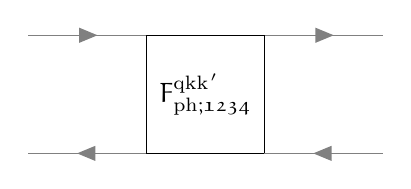
\begin{tikzpicture}[baseline=(current bounding box.center)]
	\begin{feynman}
		\vertex (a1);
		\vertex[below=of a1] (a2);
		\vertex[right=of a1] (b1);
		\vertex[below=of b1] (b2);
		\vertex[right=of b1] (c1);
		\vertex[below=of c1] (c2);
		\vertex[right=of c1] (d1);
		\vertex[below=of d1] (d2);
		
		\node (content) at ($(b1)!0.5!(c2)$) {$F_{\text{ph};\mathfrak{1234}}^{\q\k\kp}$};
		
		\diagram* {
			(a1) -- [fermion, gray] (b1) -- (c1) -- [fermion, gray] (d1),
			(d2) -- [fermion, gray] (c2) -- (b2) -- [fermion, gray] (a2),
			(b1) -- (b2),
			(c1) -- (c2)
		};	
	\end{feynman}
\end{tikzpicture}
\begin{tikzpicture}[baseline=(current bounding box.center)]
	\node {$=$};
\end{tikzpicture}
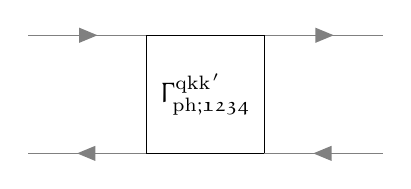
\begin{tikzpicture}[baseline=(current bounding box.center)]
	\begin{feynman}
		\vertex (a1);
		\vertex[below=of a1] (a2);
		\vertex[right=of a1] (b1);
		\vertex[below=of b1] (b2);
		\vertex[right=of b1] (c1);
		\vertex[below=of c1] (c2);
		\vertex[right=of c1] (d1);
		\vertex[below=of d1] (d2);
		
		\node (content) at ($(b1)!0.5!(c2)$) {$\Gamma_{\text{ph};\mathfrak{1234}}^{\q\k\kp}$};
		
		\diagram* {
			(a1) -- [fermion, gray] (b1) -- (c1) -- [fermion, gray] (d1),
			(d2) -- [fermion, gray] (c2) -- (b2) -- [fermion, gray] (a2),
			(b1) -- (b2),
			(c1) -- (c2)
		};	
	\end{feynman}
\end{tikzpicture}
\begin{tikzpicture}[baseline=(current bounding box.center)]
	\node {$+$};
\end{tikzpicture}
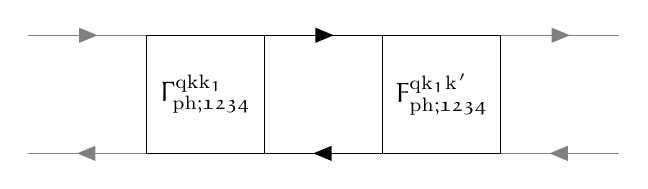
\begin{tikzpicture}[baseline=(current bounding box.center)]
	\begin{feynman}
		\vertex (a1);
		\vertex[below=of a1] (a2);
		\vertex[right=of a1] (b1);
		\vertex[below=of b1] (b2);
		\vertex[right=of b1] (c1);
		\vertex[below=of c1] (c2);
		\vertex[right=of c1] (d1);
		\vertex[below=of d1] (d2);
		\vertex[right=of d1] (e1);
		\vertex[below=of e1] (e2);
		\vertex[right=of e1] (f1);
		\vertex[below=of f1] (f2);
		
		\node (content) at ($(b1)!0.5!(c2)$) {$\Gamma_{\text{ph};\mathfrak{1234}}^{\q\k\k_1}$};
		\node (content) at ($(d1)!0.5!(e2)$) {$F_{\text{ph};\mathfrak{1234}}^{\q\k_1\kp}$};
		
		\diagram* {
			(a1) -- [fermion, gray] (b1),
			(c1) -- [fermion] (d1),
			(e1) -- [fermion, gray] (f1),
			(f2) -- [fermion, gray] (e2),
			(d2) -- [fermion] (c2),
			(b2) -- [fermion, gray,] (a2),
			(b1) -- (b2),
			(b1) -- (c1),
			(b2) -- (c2),
			(c1) -- (c2),
			(d1) -- (e1),
			(d2) -- (e2),
			(d1) -- (d2),
			(e1) -- (e2),
		};	
	\end{feynman}
\end{tikzpicture}


\end{document}